\chapter{Background}
\label{chapter:background}
\minitoc

Content sharing is currently an universal concern among computer users and has recently become an important requirement for mobile devices. Indeed, thanks to the efficient wireless connectivity offered by mobile devices, users are frequently brought to locate and share content of interest (photos, videos, etc) with other members of the same spontaneous community. With current technologies, they are mainly using point-to-point basic connections, which can be considered as an efficient solution when the number of users interested in the sharing session is very small and that there is no possible connexion disruption. However, even with a guaranteed wireless connexion (Ad-Hoc network) and in the case of a large community (for example, mobile devices users assisting to a conference and willing to share some papers), one is facing the following problem: Increasing the number parallel point-to-point communications may decrease the global Ad-Hoc network capacity, while increasing dramatically the download time. The multi-hop point-to-point communication over long paths is also a serious issue. Therefore, there is a strong need to organize the communication overlay among devices in a way to distribute fairly the burden of content sharing among the set of participants while aiming to decrease the global download time. P2P file sharing solutions are good candidates for such infra-structureless networks (MANET) as they are based on multi-sourcing which balances resource consumption among users and reduces the dependency on any central entity. But unfortunately, P2P content sharing applications developed for the Internet cannot directly be plugged and used into mobile devices. Indeed, on one hand, these solutions are not adapted to the constraints of multi-hop wireless networks. For example, it is known that in a resource constrained environment, the choice of the users to whom to connect cannot be done independently of information on the underlying dynamic topology. Moreover, centralized users management approaches like the centralized tracker used in BitTorrent do not perform well in such environment as the tracker can be either far away or even invisible by some users because of disconnections. Furthermore, computer users rely on Internet search engines and dedicated desktop applications to look for the content they are willing to share. This approach becomes obsolete in the case of a spontaneous MANET based community and thus, a dedicated distributed content discovery approach must be provided. 

Then, if we consider a more general/challenging mobile environment where the topology is unstable and users' contact can be disrupted frequently (for example, mobile devices users moving in the street), users cannot rely any more on the content dissemination systems proposed for conventional MANETs~\cite{BitHoc}~\cite{BlueTorrent}. Indeed, the later ones are built based on the assumption that the network path are almost stable and that content providers and content consumers are connected to the same part of the network at the same time. Therefore, they are not suitable for disruption tolerant environment. From this perspective and to allow some services to operate even under
these challenging conditions, researchers have proposed a new networking paradigm, often referred to as Disruption Tolerant Networking, based on the store-carry-
and-forward routing principle. Devices there, rather than dropping a session (and respective packets) when no forwarding opportunity is available, store and carry
content until new communication opportunities arise. 

This Chapter describes the background behind our work. We start by presenting BitHoc, an open-source standalone content sharing solution that we proposed and developed for MANETs and we detail the reasons that prevent users from adopting BitHoc as a content dissemination solution in the context of a disruption tolerant environment. Then we give an overview of already exisiting solutions for content routing in a disruption tolerant environment (both point-to-point content routing and poit-to-multipoint routing protocols) and we detail the limitations of the different proposed approaches which we were able to overcome throught the architectures we are proposing in this thesis.

\section{BitHoc: A Content Sharing Solution for MANET}

In this section, we described our solution for content sharing in wireless Ad-Hoc networks. It contains three components: a distributed membership management service, a content search engine and an optimized content sharing service. The design of these services takes into consideration the constraints of mobile environments and the user needs. With the help of a real test-bed composed of PDAs and Smartphones, we were able to validate our solution in a real scenario and to compare it to other classical approaches. The experiments show that our application outperforms the classical approach and highlight the utility of its features. In particular, we were able to reduce by a factor of $2$ to $3$ the download time and to increase dramatically the sharing ratio. We designed our package in such a way to be standalone. So, the user has just to install the software to start publishing and discovering contents and sharing them later with those having the same interest. The wireless nodes not interested by the same content collaborate by forwarding packets at the routing level. Through BitHoc, we provide solutions to the following problems:

\begin{itemize}
\item{In the classical version of BitTorrent \cite{RefBT}, peers periodically contact a central rendezvous point called Tracker to obtain fresh information about the peers interested in a specific content and to update their information on the progress of the download. This membership information is dynamic since peers can join and leave the content sharing overlay (called torrent) at any time during the session. Because of the inappropriateness and the large overhead of client/server architectures in wireless Ad-Hoc networks, it is important to introduce a distributed Trackerless solution to manage the membership of the sharing session. The BitHoc tracker component of our architecture is designed for this purpose and is inspired from the membership management protocol we presented in details in~\cite{BitHoc}.}
\item{The classical version of BitTorrent \cite{RefBT} supposes that the cost of sending data packets to peers is in somehow independent of their locations. In an Ad-Hoc network, performance metrics like achievable throughput, delay, and energy consumption strongly depend on the number of hops to the peer node. So, it is clearly suboptimal and even unrealistic to deal with peers without considering the underlying topology. Furthermore, when applying the classical BitTorrent incentives in a wireless multi-hop network, nodes fail to reciprocate data fairly among them. The content dissemination scheme is close to a wave transferring data from the initial seed to the farthest peers. Through new peer selection and content piece scheduling strategies, our solution is topology-aware and ensures fair sharing. These strategies are described in details in~\cite{BitHoc}}
\item{To join a sharing session, a user should find and download the Torrent file related to that session. In the Internet, peers usually find their torrent files by the help of search engines which mainly look for the files in different central servers. This method does not apply in a mobile Ad-Hoc environment as MANETs. The BitHoc search engine overcomes this challenge by maintaining a distributed torrent file database thanks to the overlay constructed by the BitHoc Tracker.}
\end{itemize}

\subsection{Architecture of BitHoc}
\label{secarchitecture}

Figure \ref{figarch} depicts the principal components of this architecture and the interactions between them. We illustrate these interactions through three typical usage scenarios:

\begin{figure}[!h]
  \begin{center}
    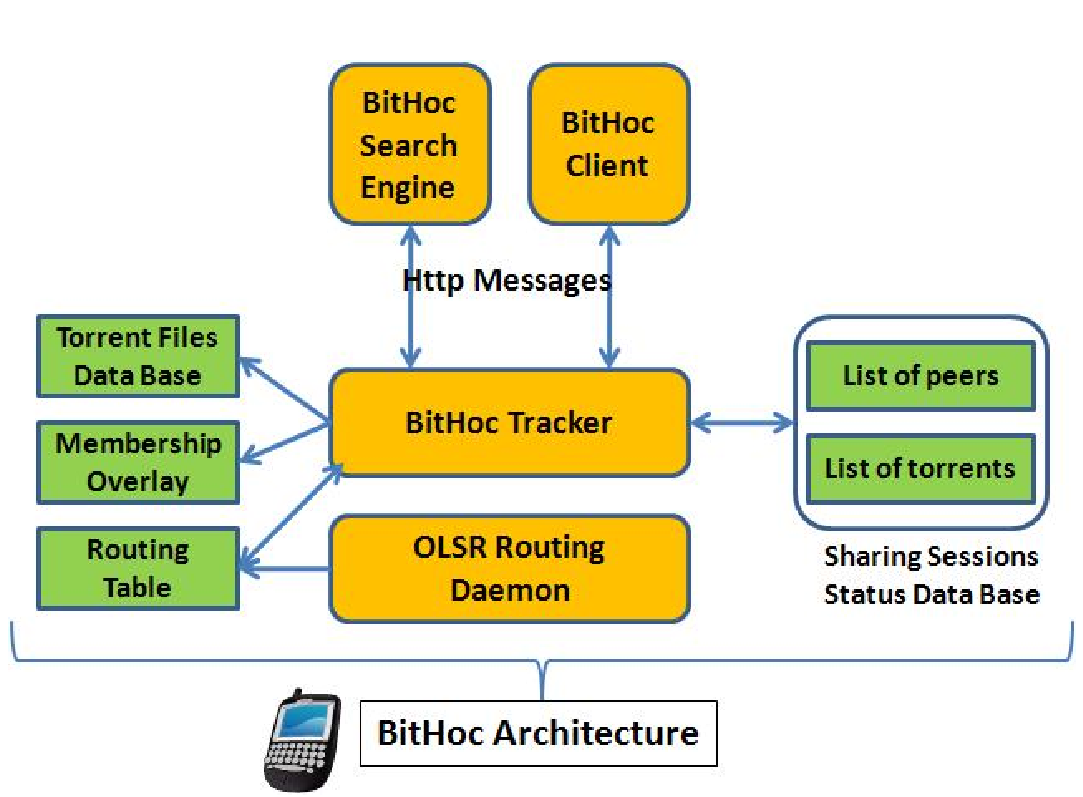
\includegraphics[width=0.7\textwidth]{Chapitre2/architecture.png}
  \end{center}
  \caption{Architecture of BitHoc}
  \label{figarch}
\end{figure}

\paragraph{Content publishing and discovery}

A user willing to share some content with the members of his community needs to indicate to the BitHoc client the location of the content in the mobile device file system. First, the client creates a meta-info file (Torrent file) that identifies in a unique manner a sharing session for this specific content. After that, the user publishes (locally) the new torrent file and a short text description of the related content using the BitHoc Search Engine service, which will update the local Torrent file database maintained in the underlying BitHoc Tacker via HTTP messages. A remote user, willing to share the same content, has to use the BitHoc search engine to find and download the Torrent file. He specifies for that the name of the content or some keywords related to its description. The request is sent via HTTP messages to its local tracker which looks for the closest match in its local database. If there are no matches, it forwards the HTTP request to the other trackers in the discovery overlay. Then, it presents the received results through an ergonomic user interface (see Figure \ref{Figsearchengine}). Based on the details of received answers (fitness to the search, number of peers involved in the sharing session, number of seeders, and number of lechers, etc), the user can choose the torrent file to download, then start sharing the content using the BitHoc Client.

\begin{figure}[!h]
  \begin{center}
    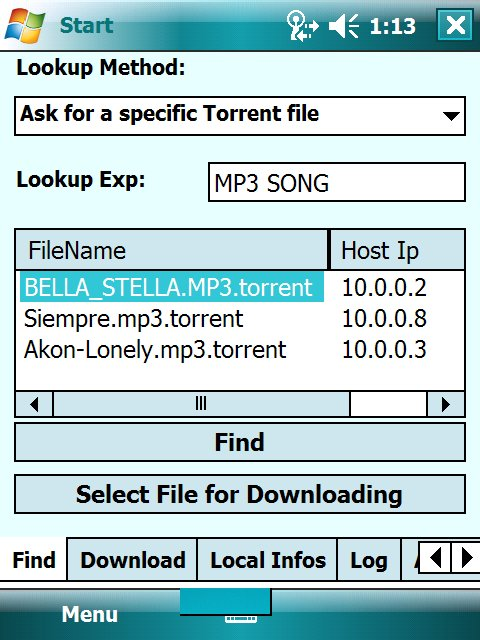
\includegraphics[width=2in,height=3in]{Chapitre2/searchengine.png}
  \end{center}
  \caption{Search Engine screen shot}
  \label{Figsearchengine}
\end{figure}

\paragraph{Membership management}

When a peer wants to join or leave the sharing session, the BitHoc client informs the BitHoc Tracker about this event using a specific HTTP message. This local agent disseminates this modification to the other BitHoc Tracker agents in other nodes in order to update their knowledge about the global membership information. The communications between Tracker agents are established in an event-driven fashion and use HTTP messages. Each tracker holds a HTTP server accepting HTTP requests from other agents and from the local BitTorrent client. The BitHoc Tracker component receives from the routing daemon up-to-date routing entries. In our testbed, the dynamics of the Ad-Hoc network are captured by the OLSR routing protocol \cite{OLSR}. Each time the number of hops toward a given peer changes, the routing daemon fires an event, which will be caught by the BitHoc Tracker and forwarded internally to the BitHoc client. This way we are sure the peer selection strategy always uses the updated number of hops to other peers. The parameters of the communications among tracker agents like HTTP listening ports and IP addresses can easily be configured by users via an ergonomic GUI. In addition to these functionalities, the BitHoc Tracker allows the user to monitor in real-time the status of the overlay (Contents it shares, members of the session, current topology of the Ad-Hoc network). He can even decide to keep traces about all the events in a file. For this, he just needs to activate the tracing option provided by the application.

\paragraph{Content sharing}

Before starting a new sharing session, the user can choose between two versions of BitTorrent algorithms: The classical version \cite{RefBT} and our version adapted to mobile Ad-Hoc networks described in~\cite{BitHoc}. The BitHoc client offers a Wizard allowing the user to configure the parameters of BitTorrent (communication ports, choking slot duration, minimum and maximum number of peers, etc). Once the torrent file is obtained, the BitHoc client can start the sharing session where it can either play the role of a leecher or a seed. It contacts periodically the local BitHoc tracker to get the current list of members of the same content sharing session (torrent). Using this list and the routing table, it manages the connections with the interested peers. Briefly a client implementing our algorithms exchanges pieces with close peers and only seeds distribute pieces across the network. Note that we allow the user to pause or resume the download while conserving the session context. He can also monitor in real time the status of the session (downloaded bytes, uploaded bytes, numbers of leechers, number of seeders, elapsed time, etc). Furthermore, the BitHoc client keeps in a log file statistics on the content sharing session and provides different levels of event traces. It also manages the storage of the downloaded contents and their classification. Figure \ref{Figclient} shows a screen-shot of the BitHoc client.

\begin{figure}[!h]
  \begin{center}
    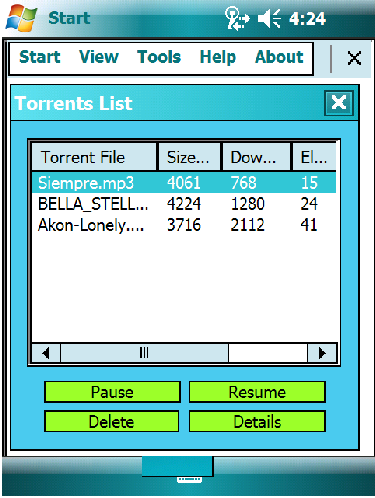
\includegraphics[width=2in,height=3in]{Chapitre2/contentsharing.png}
  \end{center}
  \caption{BitHoc Client screen shot}
  \label{Figclient}
\end{figure}

\subsection{Experimentation and results}
\label{sectest}

\paragraph{Test-bed description}

Our wireless Ad-Hoc network experimental environment consists of 14 mobile devices including 7 PDAs (HP iPAQ 214) and 7 smartphones (HP iPAQ 614c). Each handheld is equipped with an IEEE802.11b wireless card. The characteristics of the two types of devices are detailed in Table \ref{tabcarac}. The Ad-Hoc connectivity is maintained thanks to OLSR daemons run by the different devices. In our experiments, we constructed several network topologies containing a maximum of 6 hops. The objective of the realized swarm was to download a 4 MB MP-3 content. All PDAs were supposed to participate to the sharing of the file. The original seed of the content was chosen randomly among the set of the 14 PDAs.

\begin{table}[!h]
\center
\label{tabcarac}
\caption{Characteristics of mobile handhelds}
\begin{tabular}{|l|c|c|}
  \hline
   & \textbf{PDA} & \textbf{Smartphone} \\
  \hline
  \textbf{Name} & HP iPAQ 214 & HP iPAQ 614c\\
\hline
  \textbf{Processor speed} & 624 MHz & 520 MHz \\
  \hline
\textbf{RAM} & 128 MB & 128 MB \\
  \hline
\textbf{Operating system} & Windows Mobile 6 & Windows Mobile 6 \\
  \hline
\end{tabular}
\end{table}

\paragraph{Experimentation results}

\begin{figure}[!h]
  \begin{center}
    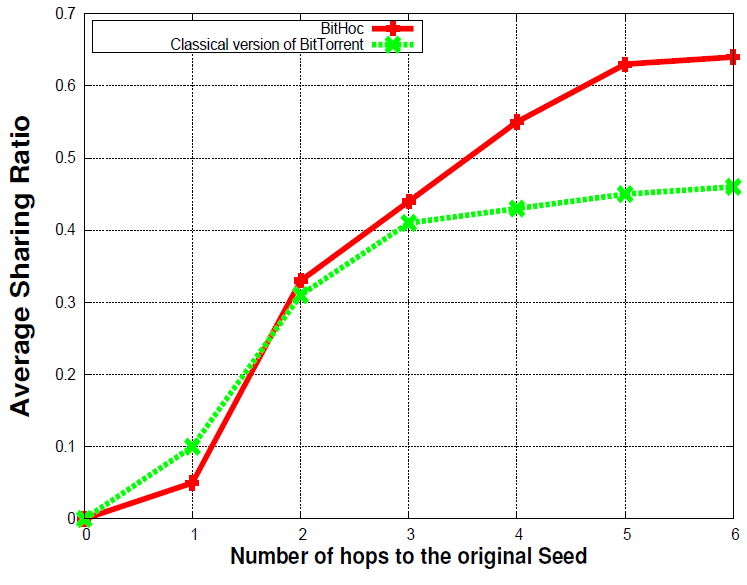
\includegraphics[width=3in,height=2.2in]{Chapitre2/sharingratio.png}
  \end{center}
  \caption{Sharing ratio}
  \label{figsharing}
\end{figure}

\begin{figure}[!h]
  \begin{center}
    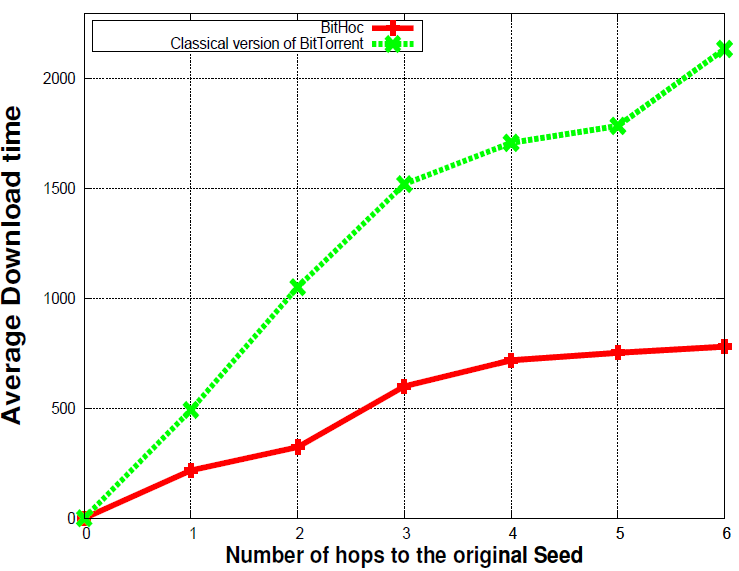
\includegraphics[width=3in,height=2.2in]{Chapitre2/downloadtime.png}
  \end{center}
  \caption{Download time}
  \label{FigDownloadtime}
\end{figure}

The metrics tracked during our experiments are the download time and the average sharing ratio of nodes. We define $R_{h}$ as the sharing ratio of peers located at $h$ hops from the original seed. It measures the level of reciprocity between downloads and uploads. In the ideal case, the ratio should be close to $1$. The two versions of BitTorrent (The legacy one and ours) have been tested and the results are presented in Figures \ref{figsharing} and \ref{FigDownloadtime}. Figure \ref{figsharing} shows a dramatic increase of sharing opportunities when our adapted version is deployed. The routing overhead generated by the classical version makes any gain obtained by important diversification of pieces negligible. Our method finds the good equilibrium between sharing and diversification. Figure \ref{FigDownloadtime} shows that BitHoc outperforms the classical version of BitTorrent in terms of download time. It is in accordance with our research results presented in~\cite{BitHocWeb}. More information about our experiments and our GPL licensed open-source code can be found on the BitHoc web site \cite{BitHocWeb}.

\subsection{BitHoc limitations with respect to a disruption prone environment}
\label{BitHoc:limitations}

We should note that BitHoc is built based on the assumptions that the network path are almost stable and that content providers and content consumers are connected to the same part of the network at the same time. Indeed, as described in Figure~\ref{figarch}, BitHoc relies on the routing table built and maintained by the OLSR MANET routing protocol towards maintaining the sharing sessions membership overlay and in order to deliver messages to peers at more than one hop. Therefore, BitHoc is not suitable solution for content dissemination in a disruption tolerant environment. 

\section{Disruption Tolerant Networks}

Delay and disruption tolerant networks (DTNs) are a new class of wireless networks that seek to address the networking issues in mobile or challenging environments that lack
continuous network connectivity. DTNs have emerged recently and are continuing to gain extensive efforts from the networking research community~\cite{Bundle,fall03,dtnrg}. In the literature, these networks are found under different terminologies such as sparse mobile ad hoc networks, extreme wireless networks, or under another commonly used term intermittently connected networks. Basically, DTNs appear in areas where the network spans over large distances with low node density and/or with high node mobility. DTNs might appear also due to short radio range, power saving mechanism at the nodes, or nodes failure. Examples of such networking scenarios include, but are not limited to :

\begin{itemize}
\item{Vehicular networks, e.g.~\cite{Levine:MaxProp, DriveThru}. In~\cite{DriveThru}, the authors propose the Drive-thru Internet architecture where the objective is to provide network and Internet connectivity
to mobile users in vehicles. The network is constituted by hot spots that are placed along the roads providing thus intermittent connectivity to the users that can
connect within proximity. In~\cite{Levine:MaxProp}, Burgess et al. introduce UMass DieselNet which is a network made of 30 buses equipped with 802.11b wireless interfaces and GPS devices. The objective of the network is to provide real DTN testbed for experimental and research studies. The buses move on regular trajectories inside the UMass Amherst campuses and surrounding areas. When two buses pass nearby, they transfer data to each other. Additionally, buses can connect to open wireless access points
along the roads.}
\item{Mobile sensor networks for environmental monitoring, e.g.~\cite{zebranet02,WirelessInfostation}. Zebranet~\cite{zebranet02} is a wireless networking architecture designed to support wildlife tracking for biology research. In ZebraNet, the network is constituted by sensor collars that are attached to zebras, which log movement patterns of the zebras, and by researchers base stations that are mounted on cars which move around sporadically. When two zebras meet, the corresponding sensors exchange collected data for a potential data delivery back to researchers base-stations. Another similar biological acquisition system has been proposed in~\cite{WirelessInfostation}, where the network is made of a set of sensors attached to whales and a set of fixed info-stations that act as collecting nodes.}
\item{Communication between rural zones in toward development countries, e.g.~\cite{Brewer:DTNdeveloping}. Examples include DakNet~\cite{Brewer:DTNdeveloping} which is a wireless ad hoc network that has the capacity to provide asynchronous Internet access to remote rural residents using motorcycles and buses to carry users email and web search messages.}
\item{Deep space networks such as the Inter-planetary network (IPN)~\cite{interplanetary03}. The interplanetary network is a network of regional Internet networks. A region is an area where the characteristics of communication are the same. An example of regions includes the terrestrial Internet as a region or a ground-to-orbit region. IPN aims to achieve end-
to-end communication through multiple regions in a disconnected, variable-delay environments.}
\item{Challenged networks such as disaster healing networks after natural disaster, travel information and advertisements dissemination systems in large cities using local transport systems, military ad hoc networks where disconnection occurs because of the war or for security reasons where some links need to be shut down from time to time.}
\end{itemize}

Generally speaking, DTNs are wireless networks that do not conform to Internet or to traditional multihop and ad hoc wireless networks underlying structures and assumptions.
In particular, they are characterized mainly by the following specific features~\cite{fall03, DTNTutorial}:

\begin{itemize}
\item{Intermittent connectivity where an end-to-end path between a given source-destination pair does not exist most of the time. Path disconnections are frequent and arise from
two main factors, namely motion and/or limited power at the nodes. Disconnection due to motion can arise when one or both nodes at the end of a communication link
move, or due to some intervening object or signal that obstruct the communication. These disconnections can be predicted, for instance when the nodes move away
according to a predetermined schedule or, an opportunistic for instance according to random walk of the nodes. Disconnections that are due to power outage result
commonly from some power saving mechanisms at the wireless devices, e.g. case of sensor networks. The latter disconnections are often predictable.}
\item{Nodes have low power capabilities and limited resources. In many DTNs, nodes are generally battery powered and/or deployed in areas lacking power infrastructure. In
some other situations, nodes have limited memory and/or processing capabilities.}
\item{Large delays which are basically due to long queuing times resulting from frequent disconnections, or from low data rate at the devices.}
\end{itemize}

\section{Content Routing in Disruption Tolerant Networks}

Due to frequent disconnections in DTNs, instantaneous end-to-end routes do not exist, and hence most of the traditional Internet and/or mobile ad hoc content routing protocols fail~\cite{Fall:DTNrouting}. However, end-to-end routes may exist over time if the nodes can take advantage of their mobility by exchanging and carrying other node messages upon meetings, and by delivering them afterward to their corresponding destinations. The latter concept has given rise to a novel routing paradigm in these networks called the store-carry-and-forward approach, in which intermediate nodes serve as relays for each other. Thus, the term "mobility-assisted routing approach" that is used in conjunction to describe these schemes.

Unfortunately, these techniques result in high latency, since packets need to be carried for long time periods before being delivered. When the delivery latency is not critical, as
the case of delay-tolerant networks, the store-carry-and-forward paradigm can prove to be adequate. For instance, this is the case when the delivery of the messages is very important, possibly more important than the delay. Basically, with the store-carry-and-forward approach, the delivery delays of packets depend on the rate at which contact opportunities are created in the network, as well as the availability of network resources, such as storage space and energy. The various studies that considered routing techniques in DTNs have examined the trade-offs between optimizing the delivery ratio and delivery delay from one side, and reducing node resource consumptions in terms of storage and battery usage from the other side. However, the intricacy of each one depends on the particularity of network environment at hand, the mobility model of the nodes, the performance objectives to attain, and other criteria.

This section will survey and classify various research works that have considered content routing schemes for DTNs. Actually, there are different approaches to categorize these schemes~\cite{Ward:RoutingSurvey, DTNRoutingSurvey06}. Hereafter, we propose a classification that is based on the content distribution method. Specifically, depending on whether these schema operate on a point-to-point basis or point-to-multipoint one.

\subsection{Point to Point Content Routing in Disruption Tolerant Networks}

We classify related existing DTN point-to-point routing protocols as those that replicate packets and those that forward only a
single copy. Epidemic routing protocols replicate packets at transfer opportunities hoping to find a path to a destination.
However, naive flooding wastes resources and can severely degrade performance. Proposed protocols attempt to limit
replication or otherwise clear useless packets in various ways: \emph{(i)} using historic meeting information~\cite{Wearable, MVRouting, Levine:MaxProp}; \emph{(ii)} re-moving useless packets using acknowledgments of delivered data~\cite{Levine:MaxProp}; \emph{(iii)} using probabilistic mobility information to infer
delivery~\cite{Haas:wdtn}; \emph{(iv)} replicating packets with a small probability~\cite{Tseng:broadcast}; \emph{(v)} using network coding~\cite{LeBoudec:wdtn} and coding with
redundancy~\cite{Fall:Sigcomm05}; and \emph{(vi)} bounding the number of replicas of a packet~\cite{Haas:wdtn,akis:wdtn,Vahdat:epidemic}.

In contrast, forwarding routing protocols maintain at most one copy of a packet in the network~\cite{Fall:DTNrouting,Waterloo:wdtn,akis:technical1}. Jain et
al.~\cite{Fall:DTNrouting} propose a forwarding algorithm to minimize the average delay of packet delivery using oracles with varying
degrees of future knowledge. Deployment experience~\cite{BalasubramanianLV07} suggests that, even for a scheduled bus service, implementing
the simplest oracle is difficult; connection opportunities are affected by many factors in practice including weather, radio
interference, and system failure. Jones et al.~\cite{Waterloo:wdtn} propose a link-state protocol based on
epidemic propagation to disseminate global knowledge, but use a single path to forward a packet. Shah et al.~\cite{Shah:datamules} and
Spyropoulos et al.~\cite{akis:technical1} present an analytical framework for
the forwarding-only case assuming a grid-based mobility model. They subsequently extend the model and propose a
replication-based protocol, Spray and Wait~\cite{akis:wdtn}. The consensus appears to be~\cite{akis:wdtn} that replicating packets can improve
performance (or security~\cite{Levine:Mobihoc07}) over just forwarding, but risk degrading performance when resources are limited.

Our position is that most existing point-to-point routing schemes does not take into consideration the impact of buffer management and scheduling policies on the performance of the underlaying system. The later issues has been largely disregarded, in comparison, by the DTN community. And thus, most routing protocols only have an incidental effect on desired performance metrics, including commonly evaluated metrics like average delay or delivery probability. For example, Spray and Wait~\cite{akis:wdtn} like many other routing protocols~\cite{Haas:wdtn,Vahdat:epidemic} that route packets using the number of replicas as the heuristic, to enhance a given routing metric, does not take explicitly into account bandwidth or storage constraints which makes the effect of their design decision on the performance of a given resource constrained network scenario unclear. Nevertheless, some works already investigated the impact of plugging simple drop policies to already exiting routing protocols, like in~\cite{Towsley:Epidemic}, Zhang et al. present an analysis of buffer constrained \emph{Epidemic} routing, and evaluate some simple drop policies like drop-front and drop-tail. The authors conclude that drop-front, and a variant of it giving priority to source messages, outperform drop-tail in the DTN context. A somewhat more extensive set of combinations of \emph{heuristic} buffer management policies and routing protocols for DTNs is evaluated in~\cite{QueuingPolicies}, confirming the performance of drop-front. In~\cite{DCopies}, Dohyung et al. present a drop policy which discards a message with the largest expected number of copies first to minimize the impact of message drop. However, all these policies are also heuristic, i.e. not explicitly designed for optimality in the DTN context. Also, these works do not address scheduling. 

Yet, the combination of long-term storage and the, often expensive, message replication performed by many DTN routing protocols impose a high bandwidth and storage overhead on wireless nodes. Moreover, the data units disseminated in this context, called bundles, are self contained, application-level data units, which can often be large. As a result, it is expected that nodes' buffers, in this context, will often operate at full capacity. Similarly, the available bandwidth during a contact could be insufficient to communicate all intended messages. Consequently, we believe that regardless of the specific routing algorithm used, it is important to have: \emph{(i)} efficient drop policies to decide which content(s) should be discarded when a node's buffer is full, and \emph{(ii)} efficient scheduling policies to decide which content(s) should be chosen to exchange with another encountered node when bandwidth is limited. 

Table~\ref{RoutingSummary} shows a taxonomy of many existing DTN routing protocols based on assumptions about bandwidth available during transfer opportunities and the storage
carried by nodes; both are either finite or unlimited. For each work, we state in parentheses the mobility model used. 
$R1$ and $R2$ are important to examine for valuable insights that theoretical tractability yields but are impractical for real DTNs with limited resources. Many studies~\cite{Lindgren:probabilistic,Wearable,MVRouting} analyze the case where storage at nodes is limited, but bandwidth is unlimited ($R3$). This scenario may happen when the radios used and the duration of contacts allow
transmission of more data than can be stored by the node. However, we find this scenario to be uncommon typically storage is inexpensive and energy efficient. Trends suggest that high bitrate radios will remain more expensive and energy-intensive than storage~\cite{PRESTO}. Finally, for mobile DTNs, and especially vehicular DTNs, transfer opportunities are short-lived~\cite{Levine:MaxProp}.

\begin{table}[!h]
\renewcommand{\arraystretch}{1.1}
\caption{A classification of some related work into DTN routing scenarios}
\centering
\footnotesize
\begin{tabular}{|p{1cm}|p{1.5cm}|p{1.7cm}|p{1.5cm}|p{5cm}|}
\hline
\bfseries Cat. &\bfseries Storage &\bfseries Bandwidth  &\bfseries Routing& \bfseries Work (and mobility)\\
\hline
\bfseries R1&Unlimited & Unlimited &Replication & Epidemic~\cite{Vahdat:epidemic}, Spray and Wait~\cite{akis:wdtn}: Constraint in the form of
channel contention (Grid-based synthetic)\\
\hline
\bfseries R2&Unlimited & Unlimited &Forwarding & Modified Djikstra's algorithm Jain et al.~\cite{Fall:DTNrouting} (simple graph),
MobySpace~\cite{DTNSpace} (Powerlaw)\\
\hline
\bfseries R3&Finite & Unlimited &Replication &Davis et al.~\cite{Wearable} (Simple partitioning synthetic), SWIM~\cite{Haas:wdtn} (Ex-
ponential), MV~\cite{MVRouting}(Community-based synthetic), Prophet~\cite{prophet03}
(Community-based synthetic) \\
\hline
\bfseries R4&Finite & Finite & Forwarding& Jones et al.~\cite{Waterloo:wdtn} (AP traces), Jain et al.~\cite{Fall:DTNrouting} (Synthetic DTN topol-
ogy)\\
\hline
\bfseries R5&Finite & Finite &Replication & Our proposal (Vehicular DTN traces, testbed deployment), RAPID~\cite{Levine:Sigcomm07} (Vehicular DTN traces, testbed deployment), MaxProp~\cite{Levine:MaxProp} (Vehicular DTN traces) \\
\hline
\end{tabular}
\label{RoutingSummary}
\end{table}

We were able to find mainly two protocols that belong to the category $R5$. The first \emph{(ii)}, Max-Prop~\cite{Levine:MaxProp} that assume limited storage and bandwidth. However, it is unclear how to optimize a specific routing metric using MaxProp, so we categorize it as an incidental routing protocol. And the second \emph{(ii)}, RAPID~\cite{BalasubramanianLV07} that is the first protocol to explicitly assume both bandwidth and (to a lesser extent) buffer constraints exist, and to handle the DTN routing problem as an optimal resource allocation problem, given some assumption regarding node mobility. As such, it is the most related to our proposal, and we will compare  directly against it. Despite the elegance of the approach, and performance benefits demonstrated compared to well-known routing protocols, RAPID suffers mainly from the following drawbacks: \emph{(i)} its policy is based on suboptimal message utilities (more on this in Section~\ref{sec:optimal-policy}); \emph{(ii)} in order to derive these utilities, RAPID requires the flooding of information about all the replicas of a given message in the queues of all nodes in the network; yet, the information propagated across the network might arrive stale to nodes (a problem that the authors also note) due to change in the number of replicas, change in the number of messages and nodes, or if the message is delivered but acknowledgements have not yet propagated in the network; and \emph{(iii)} RAPID does not address the issue of signaling overhead. Indeed, in~\cite{Levine:Sigcomm07}, the authors showed that whenever the congested level of the network starts increasing, their meta-data channel consumes more bandwidth. This is rather undesirable, as meta-data exchange can start interfering with data transmissions amplifying the effects of congestion. In another work~\cite{AOBM}, Yong et al. present a buffer management schema similar to RAPID. However they do not address the scheduling issue nor the trade-off between the control channel overhead and system performance. Through our proposal, we successfully address all these three issues.

\subsection{Point to Multi-Point Content Dissemination in Disruption Tolerant Networks}

As hilighted in the latter section, a significant share of research on opportunistic networks has focused on \emph{unicast} point-to-point content routing (see e.g.~\cite{DTNTaxonomy} or~\cite{Passarella:Survey}). Instead, in this section, we consider the problem of content dissemination. This is a key research problem, 
particularly in opportunistic networks. In this environment, according to the user-generated content wave, users are expected to generate large amounts of content 
by exploiting capability-rich mobile devices (such as PDAs, smartphones, etc.), and to share them with people around them.  The problem of efficiently disseminating contents in opportunistic networks is thus very relevant, and not widely explored in the literature yet.
 
Content dissemination in opportunistic networks is a difficult problem. As the topology is very unstable, and users appear in and disappear from the network dynamically, content providers and content consumers might be completely unaware of each other, and never connected at the same 
time to the same part of the network. Therefore, contents should be moved and replicated in the network in order to carry them to interested users despite disconnections 
and partitions. On the other hand, content dissemination systems should take care of both network and device resource constraints.
For example, a trivial solution would be to flood the whole network with any generated content, but this would clearly saturate both network resources (in terms of available bandwidth) and device resources (e.g., in terms of energy, storage, etc.). Content dissemination systems should also take care of the willingness of people to collaborate. Indeed,  
experience teaches us that selfish behavior is often the norm, unless incentives are provided, and can be a major impediment to any such peer-to-peer system in the wild~\cite{NashEquilibria}. Thus, we believe that content dissemination systems should consider users to be inherently selfish, instead of inherently collaborative and provide the necessary mechanisms to enforce collaboration and prevent the bad impact of selfish behaviors on the overall system performance.  

Content dissemination systems have been proposed for the Internet, and also for conventional MANETs~\cite{BitHoc}. In general, these systems assume that network paths are rather stable, and often generate a significant amount of traffic to maintain knowledge of other devices' caches. Therefore, they are not suitable for opportunistic networks. Table~\ref{DisseminationSummary} shows a taxonomy of most of existing DTN content dissemination systems. We classify the later systems into three categories, namely  
\emph{D1} content centric dissemination systems guided by users \emph{Interests}, \emph{D2} systems driven by users interests + social links and finally
\emph{D3}, dissemination systems guided by users interests and their locations. We also detail in Table~\ref{DisseminationSummary} whether the presented content dissemination systems provide or not needed mechanisms to handle devices' buffers management in case of congestion, contents scheduling during short lived contact opportunities and users selfishness. 

\begin{table}[!h]
\renewcommand{\arraystretch}{1.1}
\caption{A classification of content dissemination systems for DTN(s)}
\centering
\footnotesize
\begin{tabular}{|p{1cm}|p{2cm}|p{9.5cm}|}
\hline
\bfseries Cat. &\bfseries Driven by&\bfseries Work (buffer management, scheduling, users selfishness, mobility)\\
\hline
\bfseries D2&Users Interests & Our proposal, MobiTrade(handled, handled, inherently selfish, Vehicular DTN traces \& testbed deployment), DTN Podcasting by May et al.~\cite{May07wirelessopportunistic}~\cite{Lenders:Podcast}(not handled, not handled, inherently collaborative, testbed deployment), TACO-DTN by Solazzo et al.~\cite{TACODTN}(handled, handled, inherently collaborative, random waypoint), \\
\hline
\bfseries D1&Users Interests + Social Links &ContentPlace by Boldrini et al.~\cite{Chiara:MSWIM08}(handled, handled, inherently collaborative, synthetic based on the HCMM model~\cite{HCMM}), SocialCast by Helgason et al.~\cite{SocialCast2, SocialCast}(not handled, not handled, inherently collaborative, real human mobility traces + testbed deployment)\\
\hline
\bfseries D3&Users Interests + Location & Locus by Thompson et al.~\cite{LOCUS}(handled, handled, inherently collaborative, synthetic via MobiSim~\cite{MobiSim}), PeopleNet by Motani et al.~\cite{Peoplenet}(handled, not handled,inherently collaborative, random walk)\\
\hline
\end{tabular}
\label{DisseminationSummary}
\end{table}

TACO-DTN~\cite{TACODTN} by Sollazzo et al. is a time-aware approach to delay tolerant content based dissemination. It is implemented as a publish/subscribe system 
and was mainly designed to distribute temporal events to subsribed users. Temporal profiles are associated to each subscription and allow the construction of temporal 
profiles of \emph{infostations}. Events also have temporal validity. TACO-DTN uses temporal profiles in order to achieve two main tasks: \emph{(i)} buffer management, in order to decide which events to store when buffer space is limited, and \emph{(ii)} event routing, to select the right infostation or carrier on which to publish content. 

Peoplenet~\cite{Peoplenet} is hybrid system propagating and matching queries over, first, infrastructure, and, second, using DTN device-to-device communication in the wireless "last hop" (e.g. inside a cell) to forward further. It uses the  infrastructure to propagate queries of a given type to users in specific geographic locations, called \emph{bazaars}. Within each bazaar, the query is further propagated between neighboring nodes via peer-to-peer connectivity until it finds a matching query. 

BlueTorrent~\cite{BlueTorrent} is an opportunistic file sharing application for Bluetooth enabled devices that mimics BitTorent. Authors propose an index (shared contents database) dissemination and file swarming protocols for dynamic, sparse networks. The concept of distributing large files using small resumable atomic chunks is similar to our proposal. However, BlueTorrent relies on Bluetooth whereas our proposal leverages any link-layer technologies. Furthermore, we propose to structure the data in the network into channels and rely on an entirely receiver-driven content dissemination protocol.

SocialCast~\cite{SocialCast2, SocialCast} is an interest driven content distribution framework that exploits predictions based on metrics of
social interaction (e.g., patterns of movements among communities) coupled to interest-content matching mechanism to identify the best content carriers. In SocialCast, Kalman filter forecasting techniques [3] are used to predict the future evolution of the movement based on previous observations on some attributes characterizing social behavior. These predictions are used to derive an utility $U_i$ per device and interest $i$, the latter utility is used to identify whether the corresponding device is the best carrier for the contents matching the interest $i$ or not with respect to all the neighbors devices. Compared to SocialCast, our proposal uses a considerably more sophisticated utility that considers both content demand/popularity and the collaboration level of any user it encounters.

To our best knowledge, the only other work looking at pure content centric dissemination architecture for opportunistic networks is the research thread first initiated by the PodNet project~\cite{Podcasting:Secon07, May07wirelessopportunistic}. This work proposes a DTN Podcasting architecture, built around the concept of \emph{content channels}, that we also use in our proposal. In the first version of PodNet~\cite{May07wirelessopportunistic}, users only store and share channels they are interested in. So, there is no content forwarding. In a later version~\cite{Podcasting:Secon07}, simple strategies to cache other \emph{foreign} channels as well are considered, in order to force content forwarding and  improve the overall system performance. 
 
ContentPlace~\cite{ContentPlace} by Boldrini et al. attempts to improve Podcasting using explicit knowledge of social networking links of participants. The idea behind ContentPlace is to exploit social information on the environment the nodes operate, in order to enhance content dissemination. In the framework of opportunistic networks, this approach has already been successfully applied to message forwarding (e.g., \cite{Boldrini:SocialForwarding}). The idea is to
move messages closer and closer to their destinations following a path based on the social interactions between nodes. In the case of forwarding protocols, however, messages have a specific destination node, while in ContentPlace, following the user generated content 
approach, content generators might be unaware of the nodes interested in their data, and so might be the content consumers about the
nodes that generate the content they are interested in. ContentPlace provides also mechanisms to handle devices buffer congestion and content scheduling. Indeed, it assumes that users belong to social communities, and autonomically learns the time
spent by them in each community, which types of contents users of each community are interested in, and how
spread in the communities the contents are. This information is used to evaluate the utility of each encountered
content which is later used to evaluate the contents the remote peer is carrying and to select the ones that should be fetched in order to maximise the total utility of the 
contents in the local buffer. Compared to ContentPlace, our proposal does not require such user reported social information and does not make any hard assumptions regarding node mobility. 
 
Finally, the most recent work in this thread, by Hu et al~\cite{OptimalChannelChoice}, attempts a rigorous formulation of the problem of optimally matching channels (to store) to a population of devices. A distributed algorithm is then proposed based on the framework of Markov Chain Monte Carlo optimization. While we find this framework particularly interesting, it also comes at the expense of high complexity, long convergence delays (known in MCMC), and a need for carefully tuned simulated annealing~\cite{mcmc-bremaud}.

A major difference of our proposal (MobiTrade), is that we consider users to be inherently selfish, instead of inherently collaborative as in all the aforementioned studies. Experience teaches us that selfish behavior is often the norm, unless incentives are provided, and can be a major impediment to any such peer-to-peer system in the wild~\cite{NashEquilibria}. The only proposal we are aware of, dealing with selfish users in the context of DTNs is~\cite{BarterDTN}, where a Tit-For-Tat mechanism (''bartering'') is also used between nodes to exchange content. While Tit-For-Tat (TFT) ensures selfish users are blocked, it does not answer itself \emph{how collaborative nodes should optimally (re-)act in the presence of TFT}. This is answered in MobiTrade by a personalized inventory management mechanism, key to almost all the system's functions and good performance.

As a final note, MobiTrade is not a reputation system, as e.g.~\cite{Reputation}. In reputation systems, nodes collect and share their opinions about peers with others. In our case, each device forms a personal opinion of peers used to only optimize her actions. Our system is more similar to a \emph{market} of independent traders. As a result, a bad customer for device $X$ might be a good customer for device $Y$.
